\documentclass[12pt, a4paper, twoside]{article}
\usepackage[utf8]{inputenc}
\usepackage{fancyhdr}
\usepackage{graphicx}
\usepackage{caption}
\usepackage{subcaption}
\usepackage[margin=1in,footskip=0.25in]{geometry}
\usepackage{pgf}
\usepackage[absolute, overlay]{textpos}
\setlength{\TPHorizModule}{1.0 pt}
\textblockorigin{\paperwidth}{0.0 pt}

\pagestyle{fancy}
\fancyhf{}
\lhead{Mathematisches Pendel}
\rhead{Physik Bericht}


\begin{document}
    
    \pgfmathwidth{"\\\\An \\ J. Dubois \& A. Huillet\\ MNG Rämibühl\\"}
    \begin{textblock}{\pgfmathresult}[1, 0](0, 0)
    \noindent
    \\\\An \\ J. Dubois \& A. Huillet\\ MNG Rämibühl\\ 8001 Zürich
    \end{textblock}
    \begin{titlepage}
    \begin{center}
        \vspace*{1cm}
        \Huge
        \textbf{Mathematisches Pendel}
 
        \vspace{0.5cm}
        \LARGE
        Physik Kurzbericht
        \vfill
        \normalsize
        Bericht mit Bezug auf das Physikpraktikum vom 10. März 2022  
        \vspace{0.3cm}
      
        Jean \& Aurèle\\
        MNG Rämibühl\\
        24. März 2022
             
    \end{center}
 \end{titlepage}

    \newpage

    \section{Einleitung}
    Unsere Intuition würde uns sagen, dass je schneller sich ein Objekt bewegt, desto schwerer\\\\
    es ist, aber das ist eben nicht der Fall. Die direkteste und offensichtlichste Analogie\\\\
    zum Phänomen des Pendels ist das Fallenlassen von Gewichten mit unterschiedlicher\\\\
    Masse aus gleicher Höhe; beide kommen zur gleichen Zeit auf dem Boden an (ohne den\\\\
    Widerstand durch die Luftreibung zu berücksichtigen). Nehmen wir das Beispiel des \\\\
    Pendels. Nehmen wir an, wir halten das Seil, das die Masse hält, auf Armeslänge. Da\\\\
    sich kein Parameter außer einer allmählichen Zunahme der Masse ändert, wird die Kraft\\\\
    die unser Arm ausübt, um das Gewicht zu halten, immer größer.  Was wir intuitiv als\\\\
    höhere Geschwindigkeit wahrnehmen, ist in Wirklichkeit eine höhere Kraft, der wir \\\\
    entgegenwirken müssen. Es war Galileo Galilei, der berühmte Astronom, der im Jahr\\\\
    1590 das folgende Gesetz definierte: Die Anziehungskraft, die die Erde auf eine schwere\\\\
    Masse ausübt, ist stärker als die auf eine leichte Masse. Um eine schwere Masse in \\\\
    Bewegung zu setzen, ist jedoch mehr Energie erforderlich: Trägheit. Bei einem Fall \\\\
    gleichen sich Anziehung und Trägheit jedoch perfekt aus, sodass die Geschwindigkeit \\\\
    immer gleich bleibt.In der klassischen Gleichung für die Periode eines Pendels kommt \\\\ 
    die Masse übrigens nicht vor. Das Prinzip des Pendels hat viele Entdeckungen ermöglicht. \\\\
    So hat Foucault auf diese Weise die Drehbewegung der Erde nachgewiesen. Das  \\\\
    Pendel wurde auch verwendet, um die Geschwindigkeit von Geschossen in der \\\\
    Ballistik zu berechnen.
    \newpage
    \section{Theorie}
    Es existieren zwei Arten von klassischen Pendeln. Das mathematische Pendel, was die einfachste und idealste Repräsentation eines Pendels ist, und das physikalische Pendel. Es ist eine realistischere  Repräsentation, aber wir werden uns heute mit einem mathematischen Pendel beschäftigen. An einer Seile einer bestimmten Länge wird eine Masse angehängt, wobei die Masse und Dehnung der Seile so gering wie möglich sind. 
    Durch die sich wiederholende Natur der Bewegung eines Pendels ist es möglich, seine Bewegungen durch das zweite Newton’sche Gesetz auszudrücken. 
    Das Objekt, das als Masse dient, wird als Punktmasse betrachtet, und somit hat keine Grösse oder Form, und keine Reibung.\\
    Bemerkung:\\
    \[E_{kin}=\frac{1}{2}mv^{2}\] 
    \[E_{pot}=mgh\]
    \begin{figure}[h!]
        \begin{center}
            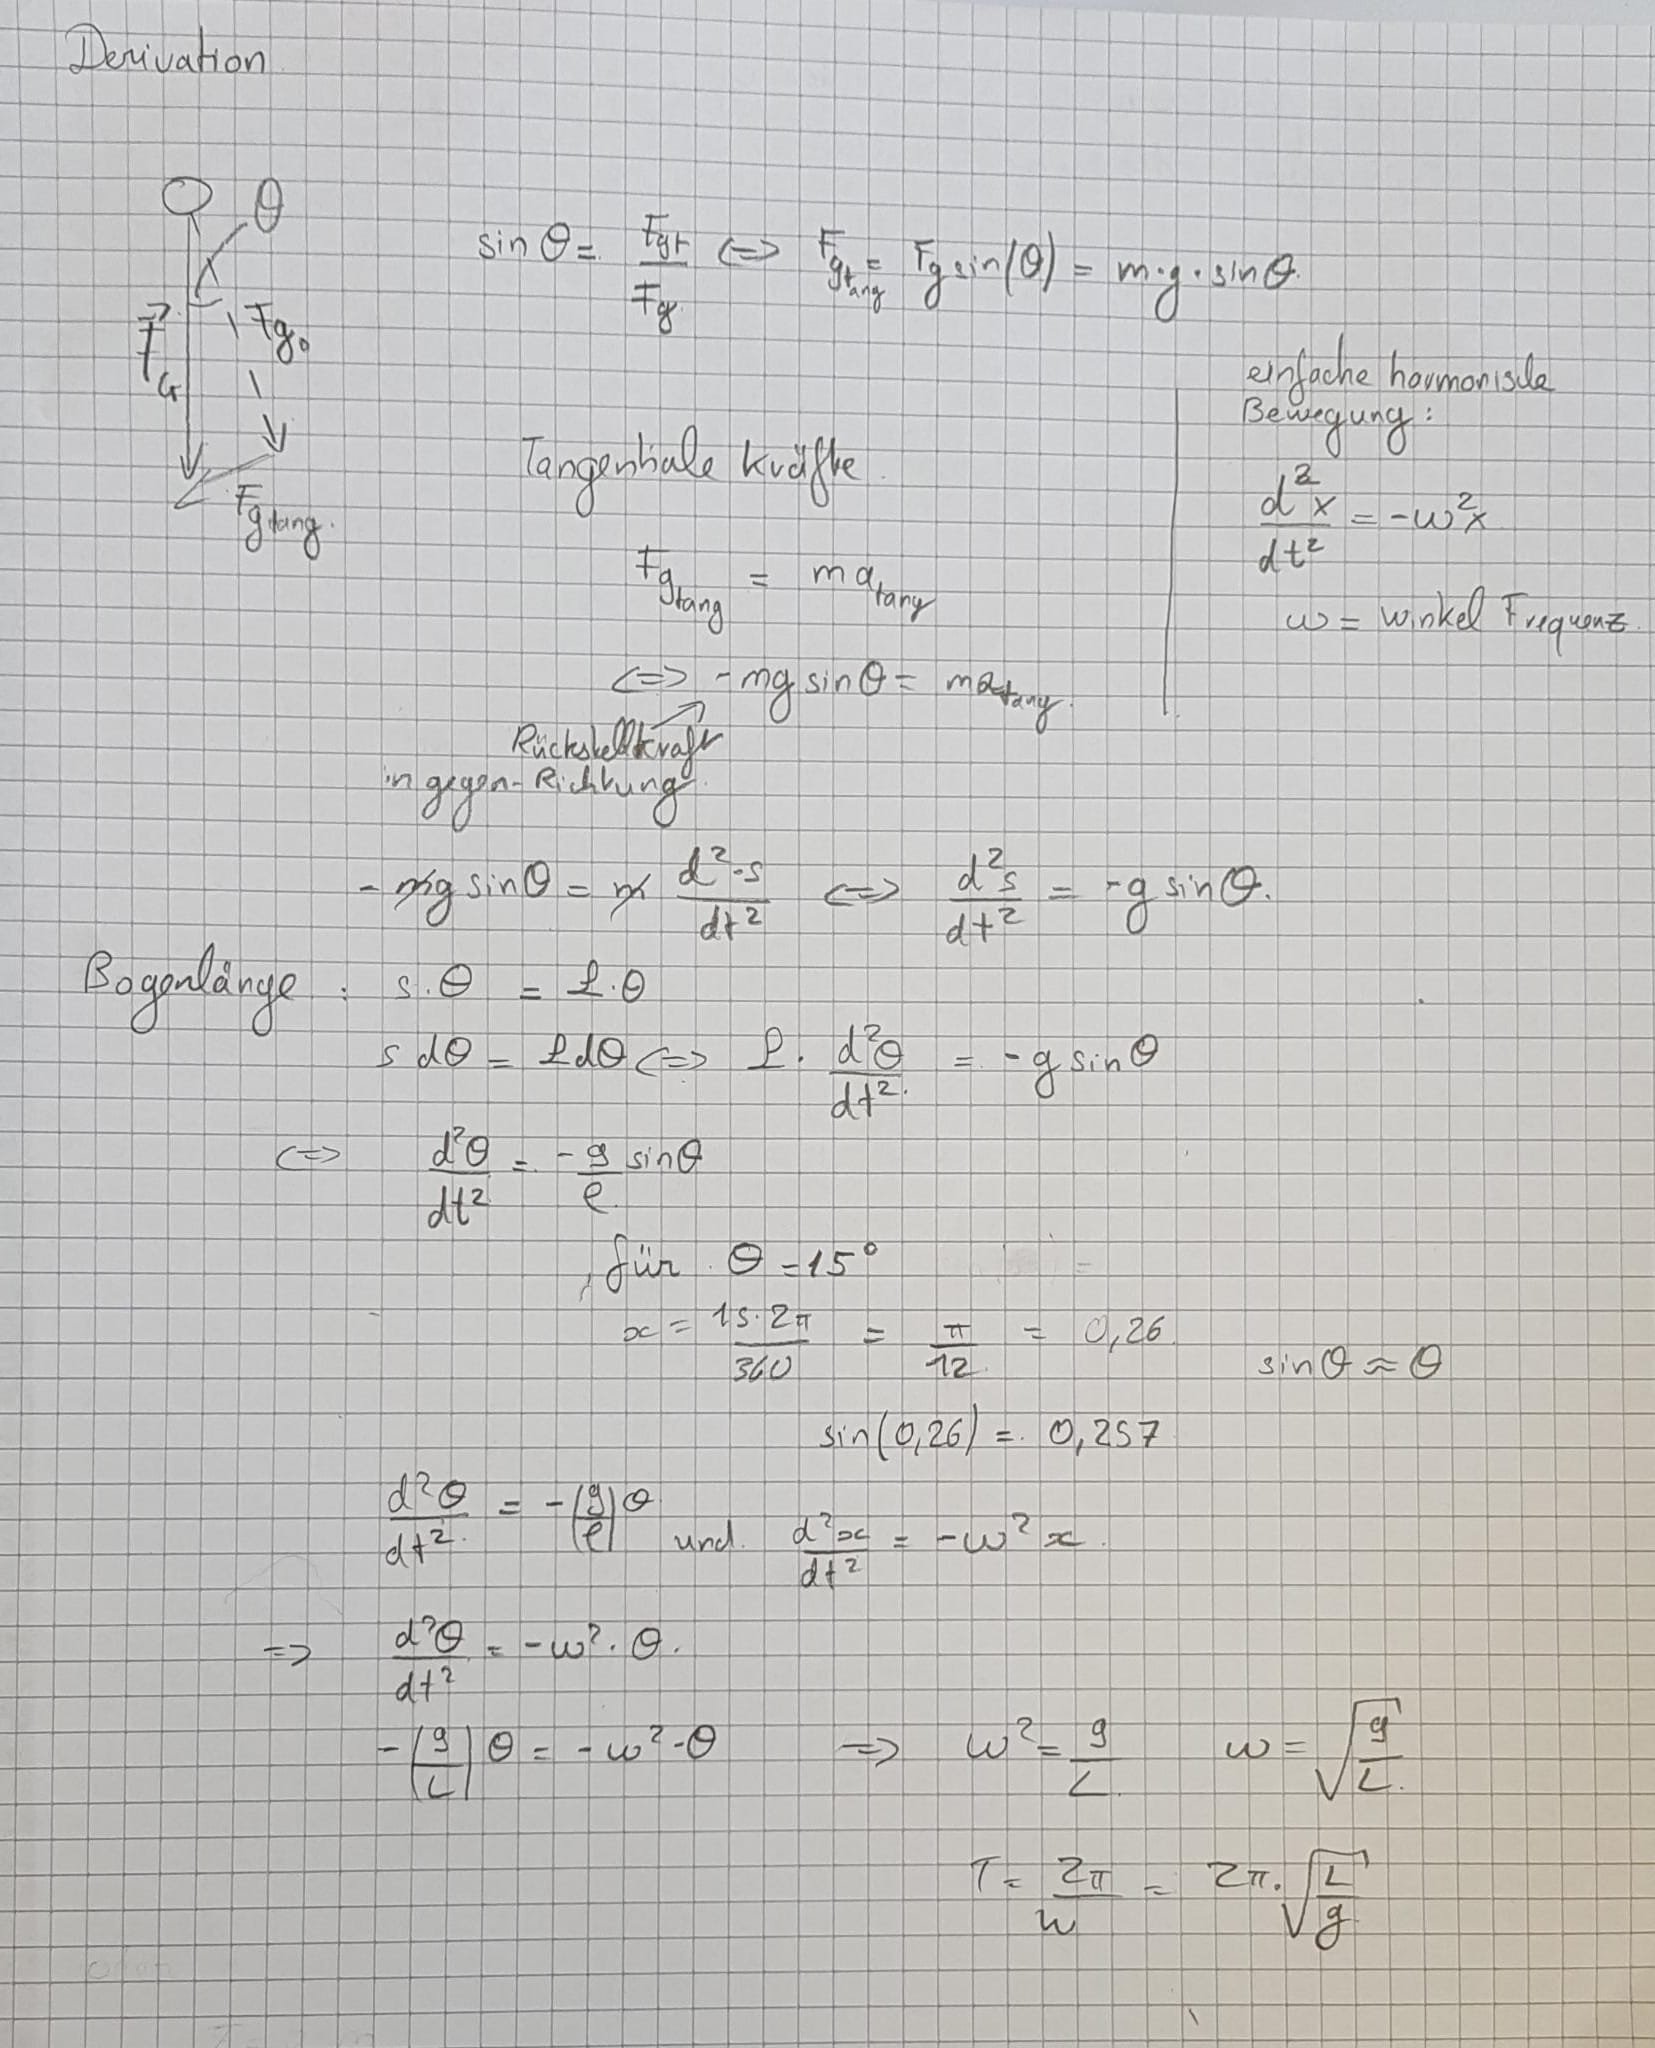
\includegraphics[scale=0.25, width=10cm]{Theorie.jpeg}
            \caption{Ableitung Gleichung Schwingungsdauer}
        \end{center}
    \end{figure}
    \newpage
    \section{Experiment}
    In unserem Experiment benutzen wir ein klassisches Pendel mit einer Masse und einer\\\\
    Seile. Oben steht einen Winkelmesser, wo die Seile im Ruhezustand bei 90 Grad steht.\\\\
    Insgesamt haben wir mit drei verschiedenen Massen, und zwei verschiedene Winkel\\\\
    gearbeitet. Die Masse wird vernachlässigt, und wir haben angenommen, dass die Seile\\\\
    keine Dehnung untergeht. Die Seilenlänge ging von 10cm bis zu 100cm, oder 1\\\\
    Meter. Die Periode wurde gemessen, jedes Mal das Pendel Vertikal zum Boden war\\\\
    (90° auf den Winkelmesser). 
    \vfill
    \begin{figure}[h!]
        \begin{subfigure}{.5\textwidth}
            \centering
            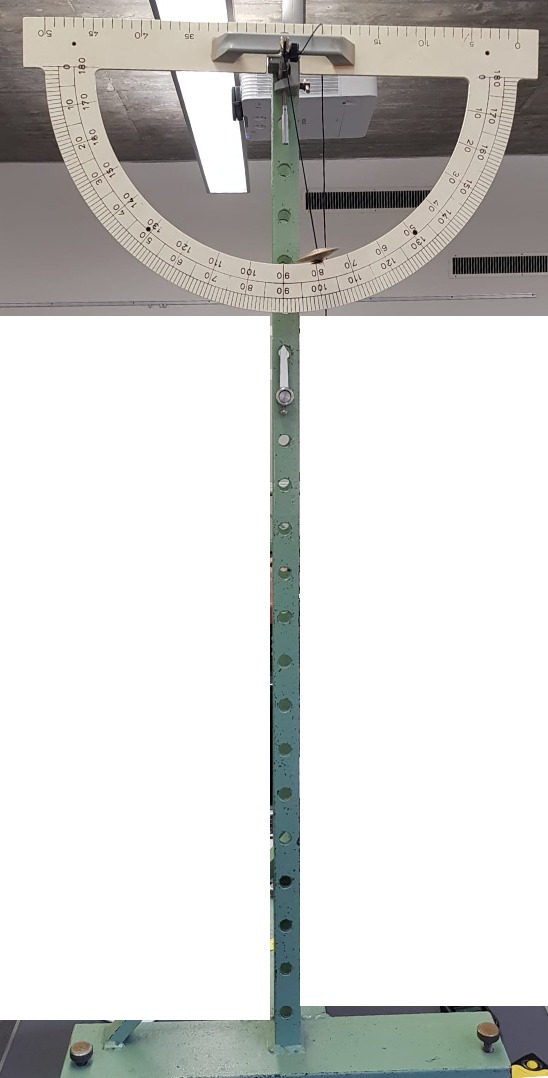
\includegraphics[scale=0.25, width=3cm]{Winkelmesser.png}
            \caption{Winkelmesser}
            \label{fig:winkelmesser}
        \end{subfigure}
        \begin{subfigure}{.5\textwidth}
            \centering
            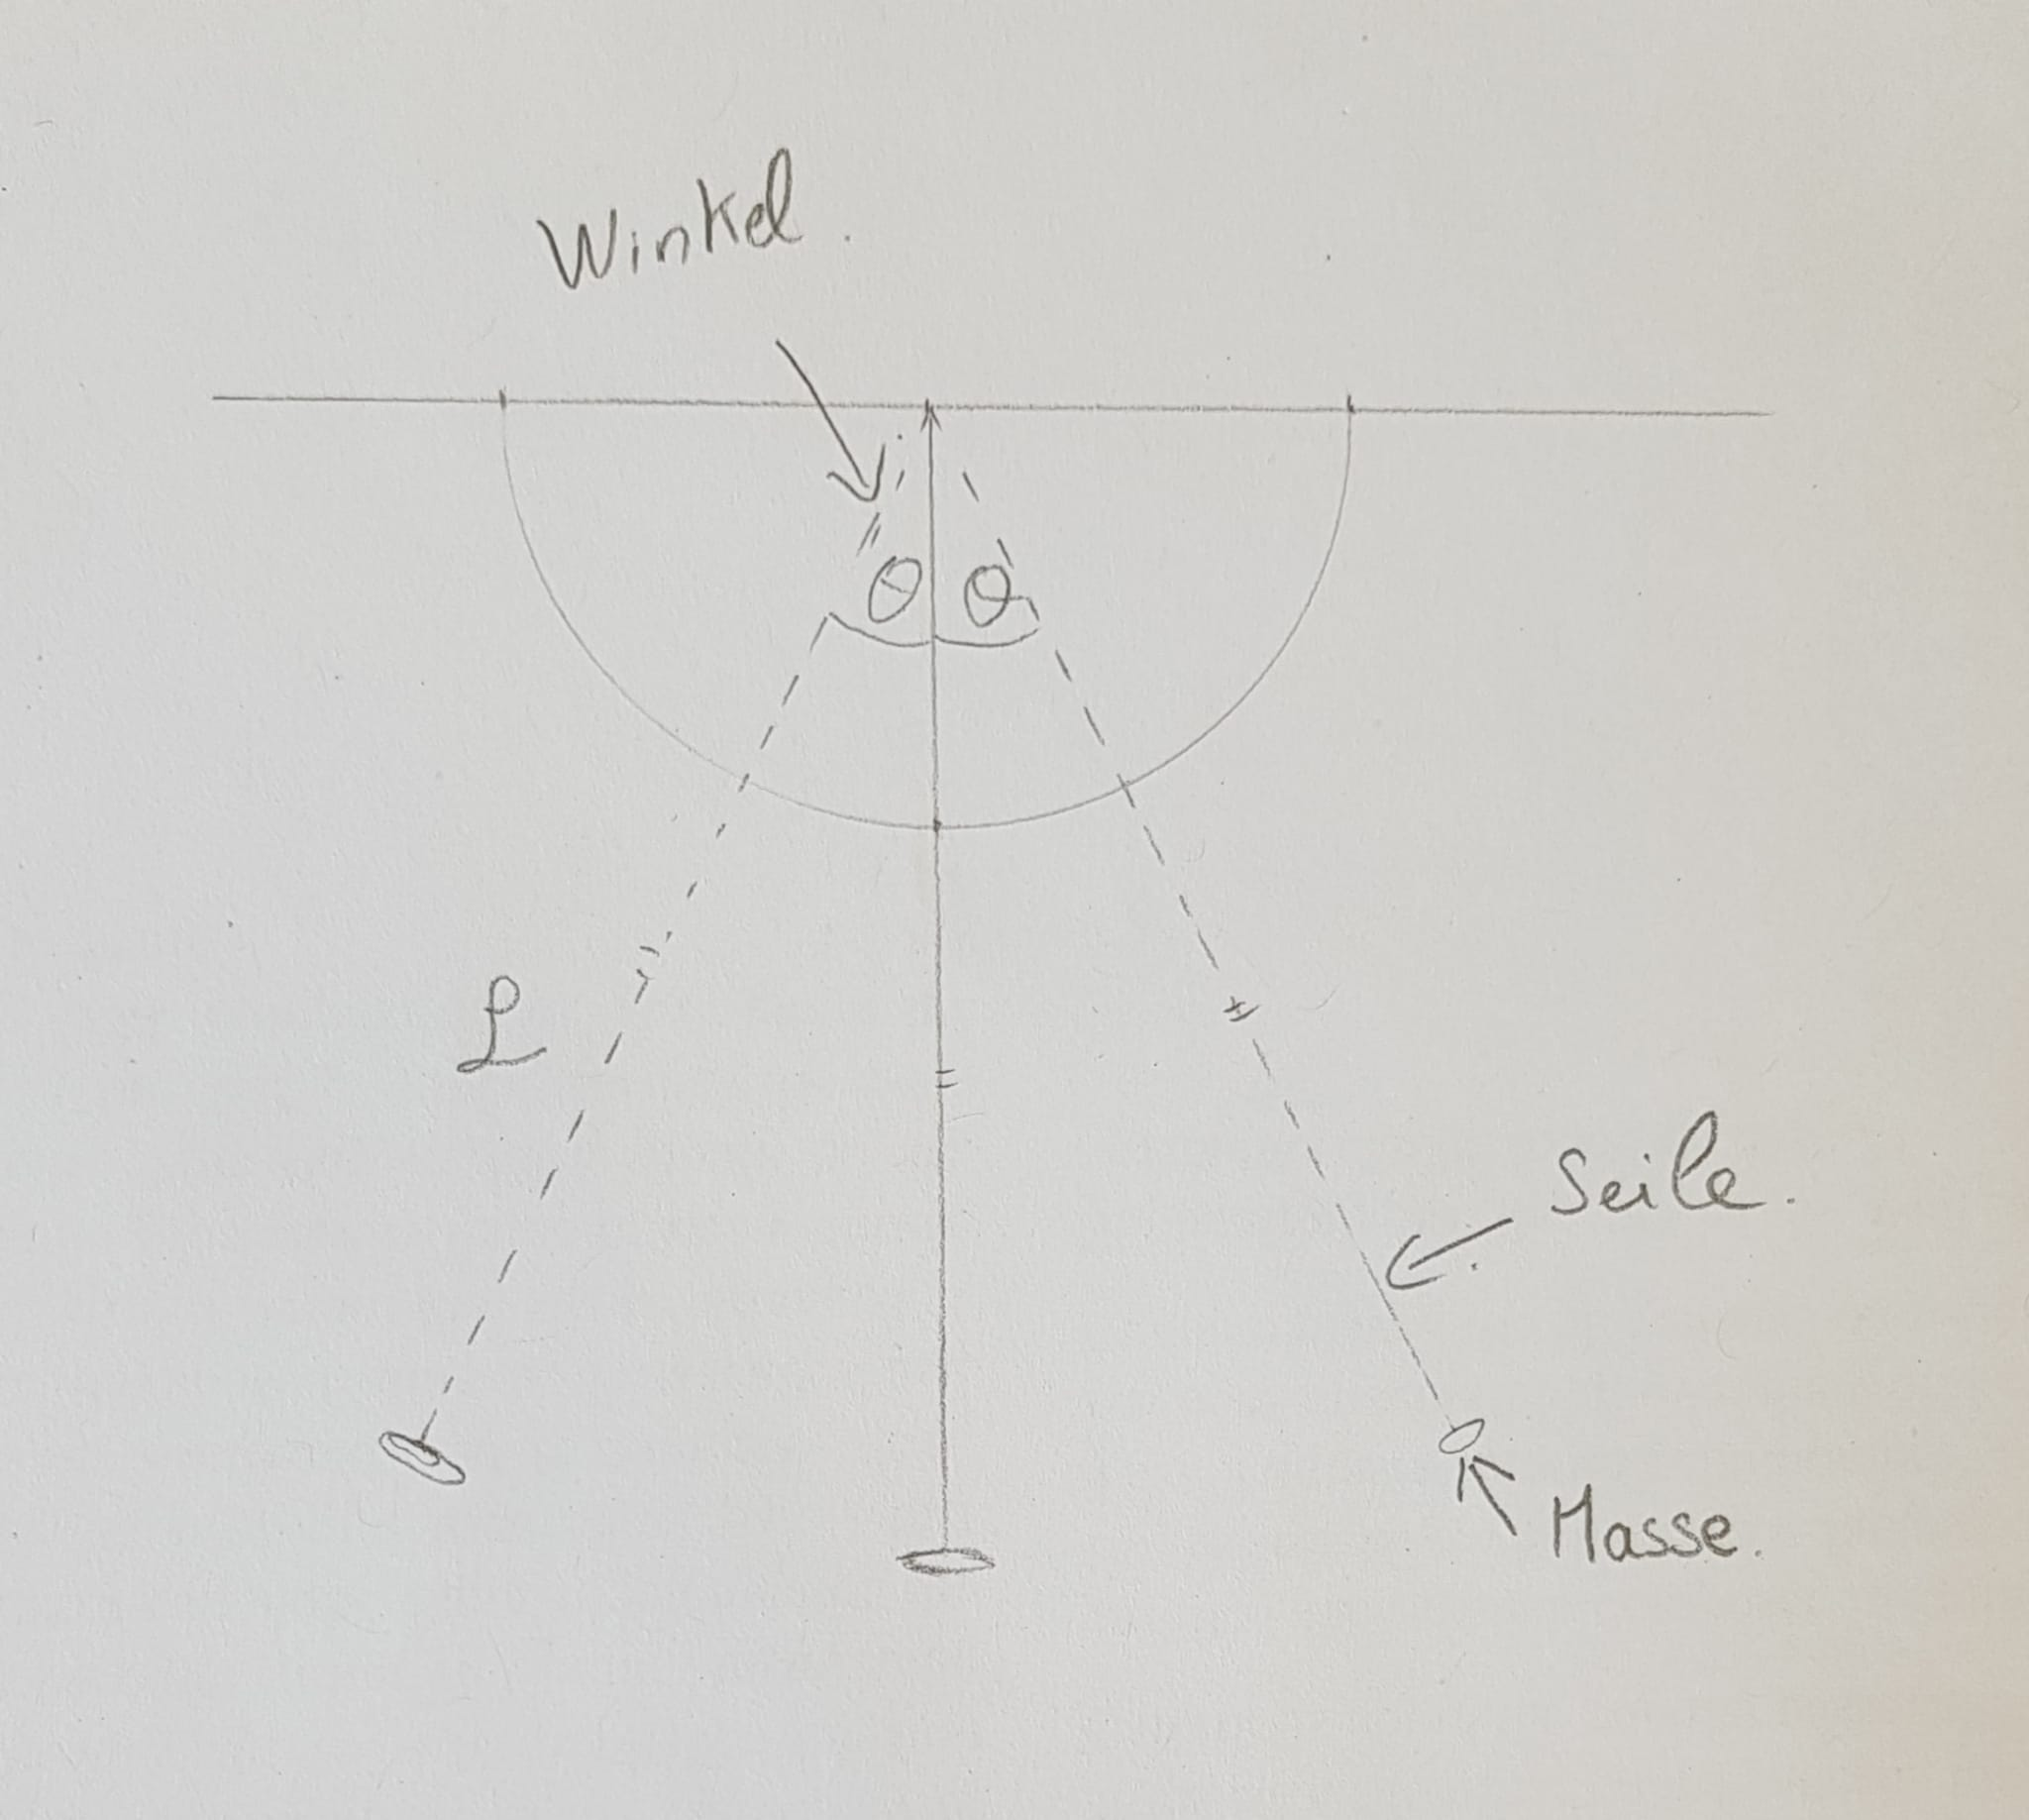
\includegraphics[scale=0.5, width=6cm]{Pendulum.jpeg}
            \caption{Skizze Pendel}
            \label{fig:Pendulum}
        \end{subfigure}
    \end{figure}
    \newpage
    \section{Bestimmung des Fehlers der Zeitmessung}
    Die Zeit für fünf Schwingungen eines Fadenpendels mit einer Amplitude von 10° wurde 20-mal berechnet. Dabei ergaben sich die folgenden Werte:
    \\
    
      \begin{center}
    \begin{tabular}{l|c|r} % <-- Alignments: 1st column left, 2nd middle and 3rd right, with vertical lines in between
      \textbf{Messung Nr.} & \textbf{Gemessene Zeit} & \textbf{Abweichung}\\
    
      \hline 
      1 & 5.86 s & 0.018 s \\
      2 & 5.88 s & 0.038 s \\
      3 & 5.88 s & 0.038 s \\
      4 & 5.81 s & 0.032 s \\
      5 & 5.83 s& 0.012 s \\
      6 & 5.82 s & 0.022 s \\
      7 & 5.83 s & 0.012 s \\
      8 & 5.78 s & 0.062 s \\
      9 & 5.86 s & 0.018 s \\
      10 & 5.78 s & 0.062 s \\
      11 & 5.92 s & 0.078 s \\
      12 & 5.78 s & 0.062 s \\
      13 & 5.81 s & 0.032 s \\
      14 & 5.83 s & 0.012 s \\
      15 & 5.91 s & 0.068 s \\
      16 & 5.81 s & 0.032 s \\
      17 & 5.89 s & 0.048 s \\
      18 & 5.87 s & 0.028 s \\
      19 & 5.84 s & 0.002 s \\
      20 & 5.85 s & 0.008 s \\

    \end{tabular}
  \end{center}
    Die mittlere Zeit für eine Schwingung entspricht also 5,842 Sekunden.
    Das Fehler der Zeitmessung beträgt 0.078 Sekunden. Dies bedeutet, dass jede Messung mindestenas 8 Sekunden dauern muss, damit der Fehler max. 1\% beträgt.
    \newpage
    \section{Messungen}
    \subsection{Messung A}
    Diese Messung besteht darin, die Schwingungsdauer bei einer konstanten \\ Amplitude und einer konstanten Pendelmasse für zehn verschiedenen Pendellängen zu bestimmen. Die Anzahl Schwingungen ist so gewählt, dass der Fehler weniger als 1\% beträgt. \\
    \\
    \begin{center}
        \begin{tabular}{l|l|c|r|r}
            \textbf{Pendellänge} & \textbf{Anzahl Schwingungen} & \textbf{1. Messung} & \textbf{2. Messung} & \textbf{Schwingungsdauer}\\ 

            \hline
            10 \textit{cm} & 13 & 8.35 \textit{s} & 8.22 \textit{s} & 0.6370 \textit{s} \\ 
            20 \textit{cm} & 10 & 9.13 \textit{s} & 8.90 \textit{s} & 0.9015 \textit{s} \\ 
            30 \textit{cm} & 9 & 10.12 \textit{s} & 10.00 \textit{s} & 1.1180 \textit{s} \\ 
            40 \textit{cm} & 8 & 10.32 \textit{s} & 10.21 \textit{s} & 1.2830 \textit{s} \\ 
            50 \textit{cm} & 9 & 12.89 \textit{s} & 12.98 \textit{s} & 1.4338 \textit{s} \\ 
            60 \textit{cm} & 6 & 9.75 \textit{s} & 9.46 \textit{s} & 1.6008 \textit{s} \\ 
            70 \textit{cm} & 6 & 10.31 \textit{s} & 10.31 \textit{s} & 1.7187 \textit{s} \\ 
            80 \textit{cm} & 5 & 9.13 \textit{s} & 9.14 \textit{s} & 1.8270 \textit{s} \\ 
            90 \textit{cm} & 5 & 9.71 \textit{s} & 9.62 \textit{s} & 1.9330 \textit{s} \\ 
            100 \textit{cm} & 5 & 10.11 \textit{s} & 10.03 \textit{s} & 2.0140 \textit{s} \\ 

          \end{tabular}
    \end{center}       
    \subsection{Messung B}
    Hier wurde mit gleicher Pendellänge und Amplitude die Schwingungsdauer von Pendeln mit drei unterschiedlichen Massen. Es wird immer noch genug lang gemessen, um ein Fehler von weniger als 1\% zu haben.
    Die Länge des Pendels \textit{l = 50 cm} und der Neigungswinkel \textit{$\alpha$ = 20°} sind fix.
    \begin{center}
        \begin{tabular}{l|l|c|r|r}
            \textbf{Pendelmasse} & \textbf{Anzahl Schwingungen} & \textbf{1. Messung} & \textbf{2. Messung} & \textbf{Schwingungsdauer}\\

            \hline
            101,5 \textit{g} & 9 & 12,85 \textit{s} & 12,98 \textit{s} & 1,435 \textit{s}\\
            358 \textit{g} & 8 & 11,20 \textit{s} & 11,20 \textit{s} & 1,40 \textit{s}\\
            33,5 \textit{g} & 8 & 11,32 \textit{s} & 11,46 \textit{s} & 1,42 \textit{s}\\
        \end{tabular}
    \end{center}

    \subsection{Messung C}
    Das Ziel dieser Messung ist es, ein Beschloss über den Einfluss der Amplitude zu ziehen. Es wurden 2 verschiedene Amplituden gewählt. Für je eine wurden zwei Messungen durchgeführt. Die Länge des Pendels \textit{l = 50 cm} und die Masse \textit{m = 358 g} sind festgelegt.
    \begin{center}
        \begin{tabular}{l|l|c|r|r}
            \textbf{Amplitude} & \textbf{Anzahl Schwingungen} & \textbf{1. Messung} & \textbf{2. Messung} & \textbf{Schwingungsdauer}\\
            \hline
            20 ° & 8 & 11,20 \textit{s} & 11,20 \textit{s} & 1,40 \textit{s}\\
            40 ° & 8 & 11,94 \textit{s} & 11,96 \textit{s} & 1,49375 \textit{s}\\
        \end{tabular}
    \end{center}
    Man stellt fest, dass wenn der Neigungswinkel sich um 20° ändert, es fast $\frac{1}{10}$ Sekunden Unterschied gibt.
    \vspace{5cm}
    \section{Aufgaben}
    \begin{figure}[h]
        \subsection{Aufgabe 2}
        Diese Aufgabe besteht darin, die Proportionalität zwischen der Schwingungsdauer und der Wurzel der Pendellänge durch eine Grafik darzustellen.
        \begin{center}
            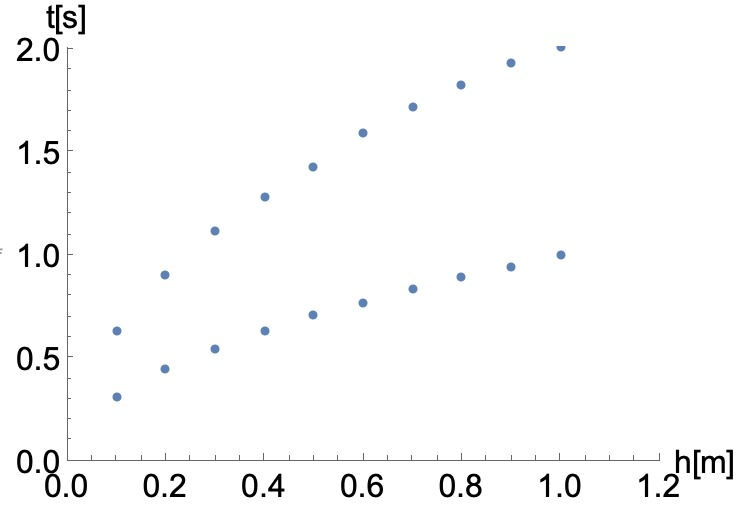
\includegraphics[width=8cm]{aufgabe2.png}
            \caption{Grafik}
        \end{center}
        Bei beiden Kurven ist die Länge die gleiche. Die obige Kurve ist durch die gemessene Zeiten dargestellt. Bei der unteren Kurve ist die Periode 
        \[T = \sqrt{l}\]
        \\Wir haben festgestellt, dass 
        \[\frac{2\pi}{\sqrt{g}} \approx 2\]
        \[2\pi \cdot \sqrt{\frac{l}{g}} \approx 2\sqrt{l}\]
    \end{figure}
        \subsection{Aufgabe 3}
        Die Regressionsfunktion entspricht (Excel):
        \[f(x)=2.00412x^{0.5054}\]
        \begin{figure}[h!]
            \begin{subfigure}{.5\textwidth}
                \centering
                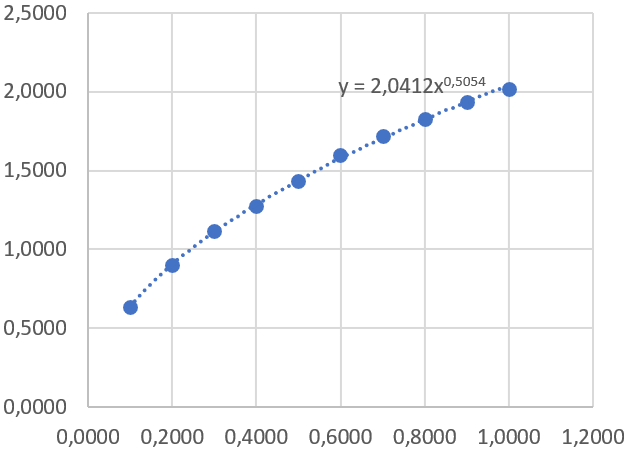
\includegraphics[scale=0.25, width=4cm]{Regression.png}
                \caption{Grafik}
                \label{fig:sub1}
            \end{subfigure}%
            \begin{subfigure}{.5\textwidth}
                \centering
                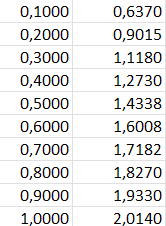
\includegraphics[scale=0.25, width=2cm]{Daten.png}
                \caption{Daten}
                \label{fig:sub2}
            \end{subfigure}
        \end{figure}
        \newpage
        Der Exponent kann aus der Formel von T hergeleitet werden:
        \[T=2\pi \sqrt{\frac{l}{g}}\]
        \[\frac{\sqrt{g}}{2\pi}\cdot T=\sqrt{l}\]
        \[\frac{\sqrt{g}}{2\pi}=\frac{\sqrt{l}}{T}\]
        \[Exp = \frac{\sqrt{l}}{T}\]

        Der Exponent entspricht also der Wurzel der Pendellänge durch die Periode.\\

        Der Regressionsfaktor kann auch aus der Formel von T herleiten:
        \[T=2\pi \sqrt{\frac{l}{g}}\]
        \[\frac{T}{\sqrt{l}}=\frac{2\pi}{\sqrt{g}}\]
        \[R=\frac{T}{\sqrt{l}}\]
        Der Regressionsfaktor entspricht also der Periode geteilt durch die Wurzel der Pendellänge.\\


        Berechnung der Fallbeschleunigung aus den berechneten Werten:
        \[T=2\pi\sqrt{\frac{l}{g}}\]     
        \[(\frac{T}{2\pi})^2=\frac{l}{g}\]
        \[g=\frac{l}{(\frac{t}{2\pi})^2}\]
        Probe mit folgende Werte:\\
        \textit{l}=10\textit{cm}; T=0.637\textit{s}
        \[\frac{0.1\textit{[m]}}{(\frac{0.637[s]}{2\pi})^2}=9.7293 [\frac{m}{s^2}]\]
        \newpage
        \section{Schlussfolgerungen}
        Mit unseren Experimenten haben wir zeigen können, dass bei gleich langen Schnuren\\\\
        aber unterschiedlichem Winkel die Periode gleich blieb. Der wichtigste Punkt, der übrigens\\\\
        unserer Intuition widerspricht, ist die Tatsache, dass die Masse keine Rolle bei der\\\\
        Periode spielt. Mit unseren erhaltenen Periodenwerten konnten wir eine\\\\
        Gravitationsbeschleunigung von 9,73 $m/s^2$  bestimmen, ein Wert, der um 1\% vom \\\\
        absoluten Wert von 9,81 $m/s^2$ abweicht, die gleiche Fehlerspanne, die wir bei unseren\\\\
        Messwerten hatten.\\\\\\
        Bei grösseren Winkeln sind die potentielle und kinetische Energie grösser, aber da die\\\\
        Bogenlänge, die die Massen folgen soll länger ist, und der Geschwindigkeit höher ist,\\\\
        gleicht sich alles heraus. Deshalb ist alles gleich bis sich die Schnurlänge ändert.\\\\\\
        Das Experiment könnte relativ einfach verbessert werden, indem man noch mehr\\\\
        Messungen macht, um präzisere Resultate zu erhalten. Andere Schnuren sowie andere \\\\
        Massen hätten untersucht sein können. Zusätzlich wurden die Limiten unseres \\\\
        Experiments, sowie der Theorie nicht untersucht. Noch besser wäre natürlich die Logik\\\\
        eines physikalischen Pendels zu folgen.
        \newpage
        \section{Literaturverzeichnis}
        \small
        FoTa 1997      Formel und Tafeln( 7.Auflage, 2019); DMK/DPK; Orell Füssli Verlag, Zürich, 1997
        


\end{document}